\documentclass{standalone}
\usepackage{tikz}
\usetikzlibrary{shapes.geometric}

\tikzset{
  shape example/.style= {color = black!30,
                         draw,
                         fill = yellow!30,
                         line width = .5cm,
                         inner xsep = 2.5cm,
                         inner ysep = 0.5cm}
}

\begin{document}

\Huge
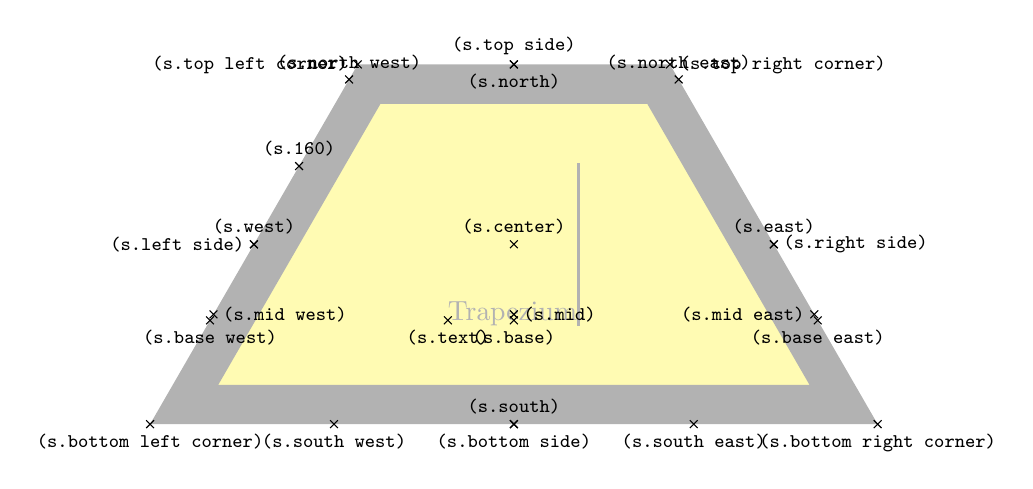
\begin{tikzpicture}
  \node[name=s, shape=trapezium, shape example, inner sep=1cm]
    {Trapezium\vrule width 1pt height 2cm};
  \foreach \anchor/\placement in
    {bottom left corner/below, top right corner/right,
     top left corner/left,     bottom right corner/below,
     bottom side/below,        left side/left,
     right side/right,         top side/above,
     center/above,   text/below,      mid/right,       base/below,
     mid west/right, base west/below, mid east/left,   base east/below,
     west/above,     east/above,      north/below,     south/above,
     north west/above, north east/above,
     south west/below, south east/below, 160/above}
  \draw[shift=(s.\anchor)] plot[mark=x] coordinates{(0,0)}
    node[\placement] {\scriptsize\texttt{(s.\anchor)}};
\end{tikzpicture}

\end{document}